\subsection{Shower Energy Sideband}
\label{sec:ShowerEnergySideband}

Two study consistency between the data and MC simulation without applying any selection criteria involving BDTs, we also employ a sideband generated through only selecting events in which the leading shower energy $> 0.75$~GeV. The results of applying the loose event selections to this sideband are shown in Figures~\ref{fig:ShrEnergySideband1eNpRuns123} and~\ref{fig:ShrEnergySideband1e0pRuns123} using data from runs 1-3, and Figures~\ref{fig:ShrEnergySideband1eNpRuns12345} and~\ref{fig:ShrEnergySideband1e0pRuns12345} using data from runs 1-5.

\begin{figure}[H]
    \centering
    \begin{subfigure}{0.5\linewidth}
        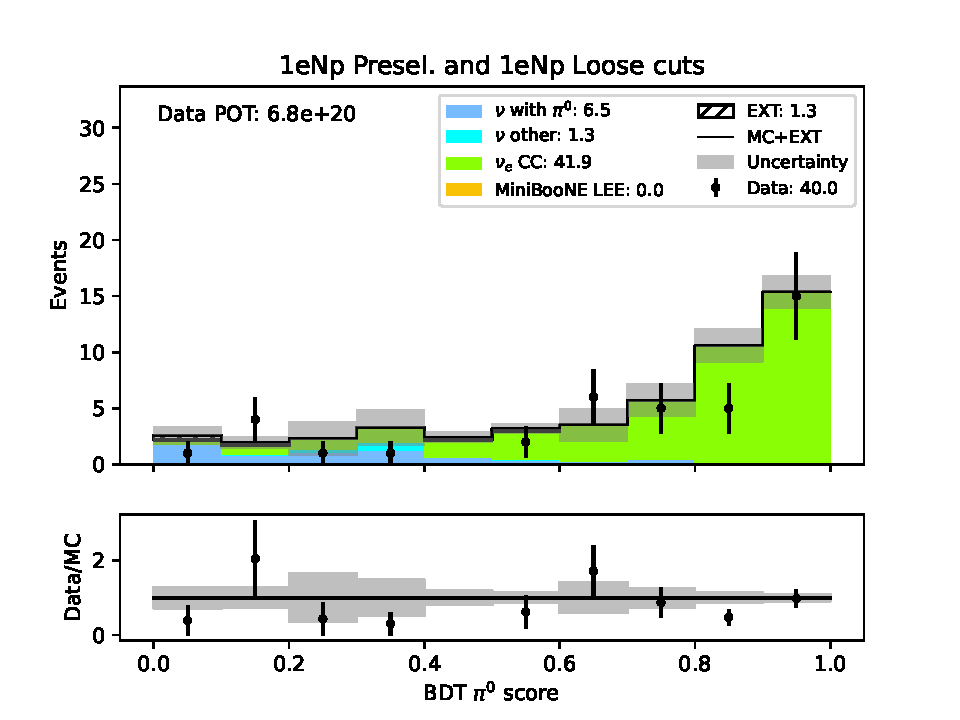
\includegraphics[width=\linewidth]{technote/Sidebands/Figures/ShowerEnergySideband/shr_energy_sideband_pi0_score_run123_NP_NPL.pdf}%
        \caption{$\pi^0$ score.}
    \end{subfigure}%
    \begin{subfigure}{0.5\linewidth}
        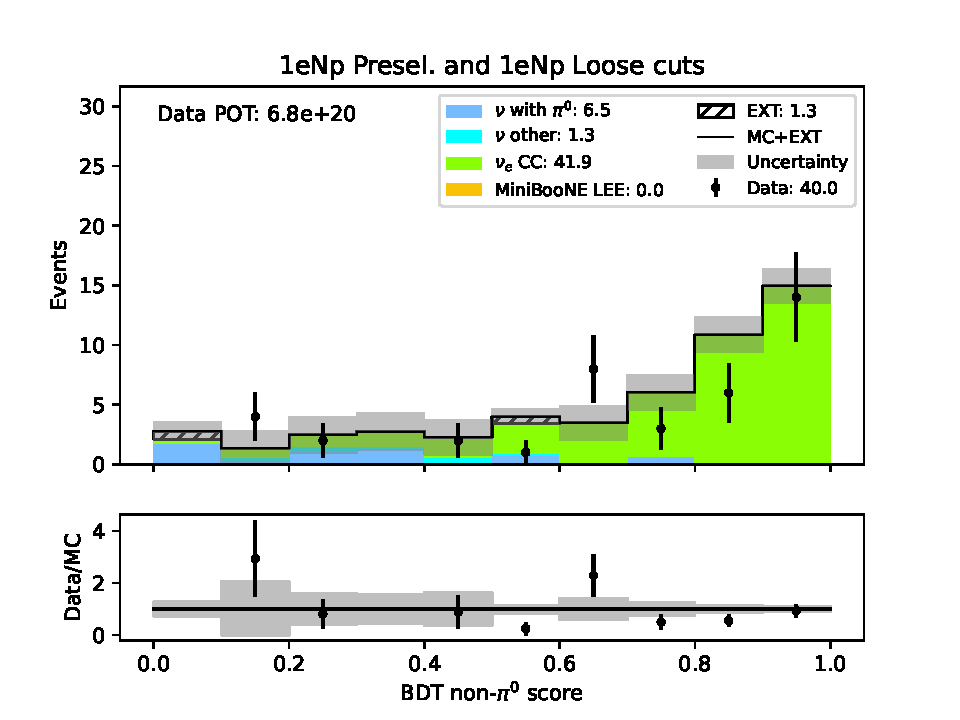
\includegraphics[width=\linewidth]{technote/Sidebands/Figures/ShowerEnergySideband/shr_energy_sideband_nonpi0_score_run123_NP_NPL.pdf}%
        \caption{Non-$\pi^0$ score.}
    \end{subfigure}
    \begin{subfigure}{0.5\linewidth}
        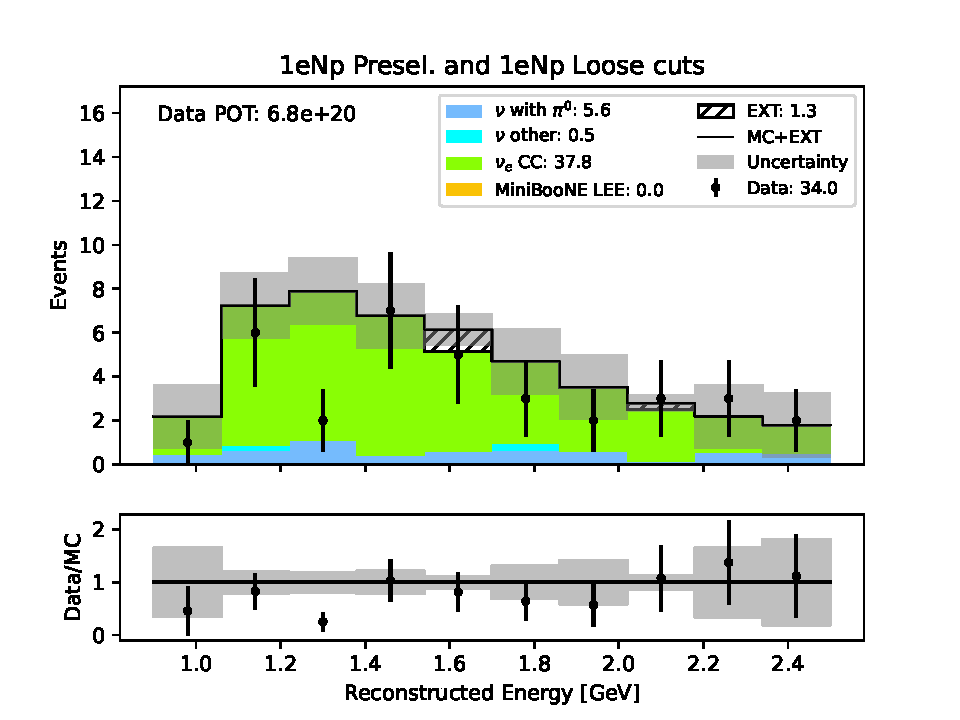
\includegraphics[width=\linewidth]{technote/Sidebands/Figures/ShowerEnergySideband/shr_energy_sideband_reco_e_run123_NP_NPL.pdf}%
        \caption{Reconstructed neutrino energy.}
    \end{subfigure}
    \caption{Results of applying the loose 1eNp event selection to the high shower energy sideband. Data from runs 1, 2, and 3 shown.}
    \label{fig:ShrEnergySideband1eNpRuns123}
\end{figure}

\begin{figure}[H]
    \centering
    \begin{subfigure}{0.5\linewidth}
        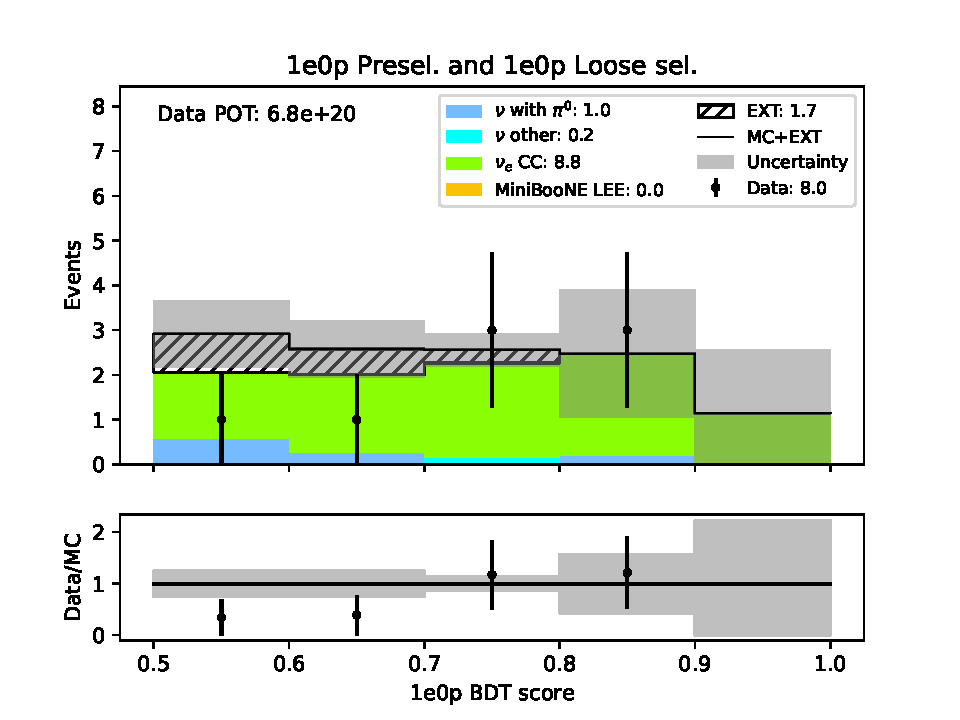
\includegraphics[width=\linewidth]{technote/Sidebands/Figures/ShowerEnergySideband/shr_energy_sideband_bkg_score_run123_ZP_ZPLOOSESEL.pdf}%
        \caption{Background score.}
    \end{subfigure}%
    \begin{subfigure}{0.5\linewidth}
        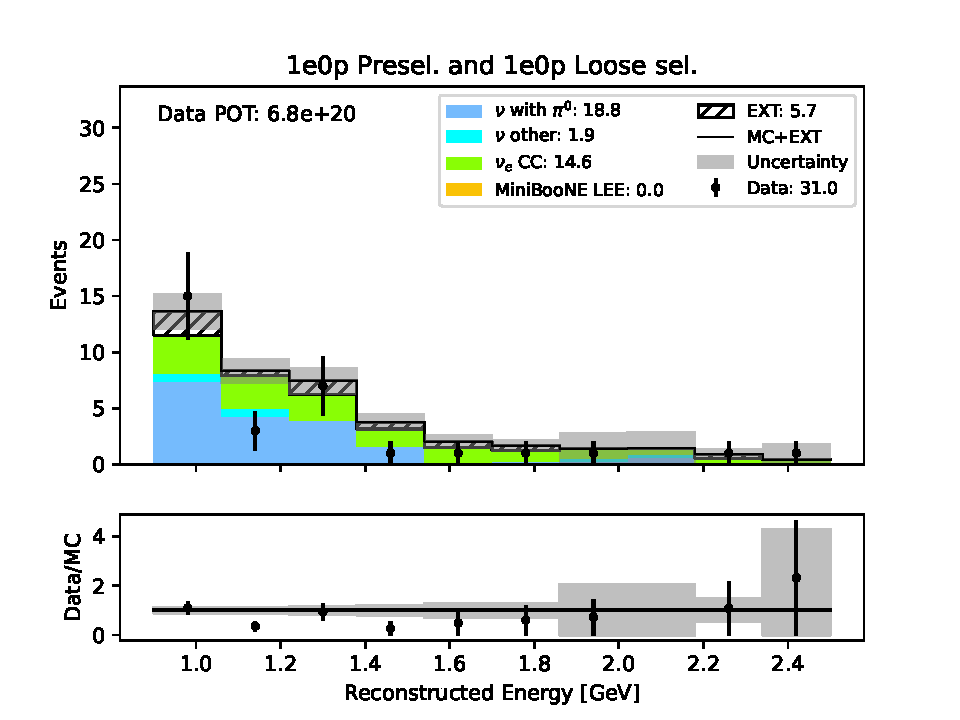
\includegraphics[width=\linewidth]{technote/Sidebands/Figures/ShowerEnergySideband/shr_energy_sideband_reco_e_run123_ZP_ZPLOOSESEL.pdf}%
        \caption{Reconstructed neutrino energy.}
    \end{subfigure}
    \caption{Results of applying the loose 1e0p event selection to the high shower energy sideband. Data from runs 1, 2, and 3 shown.}
    \label{fig:ShrEnergySideband1e0pRuns123}
\end{figure}

\begin{figure}[H]
    \centering
    \begin{subfigure}{0.5\linewidth}
        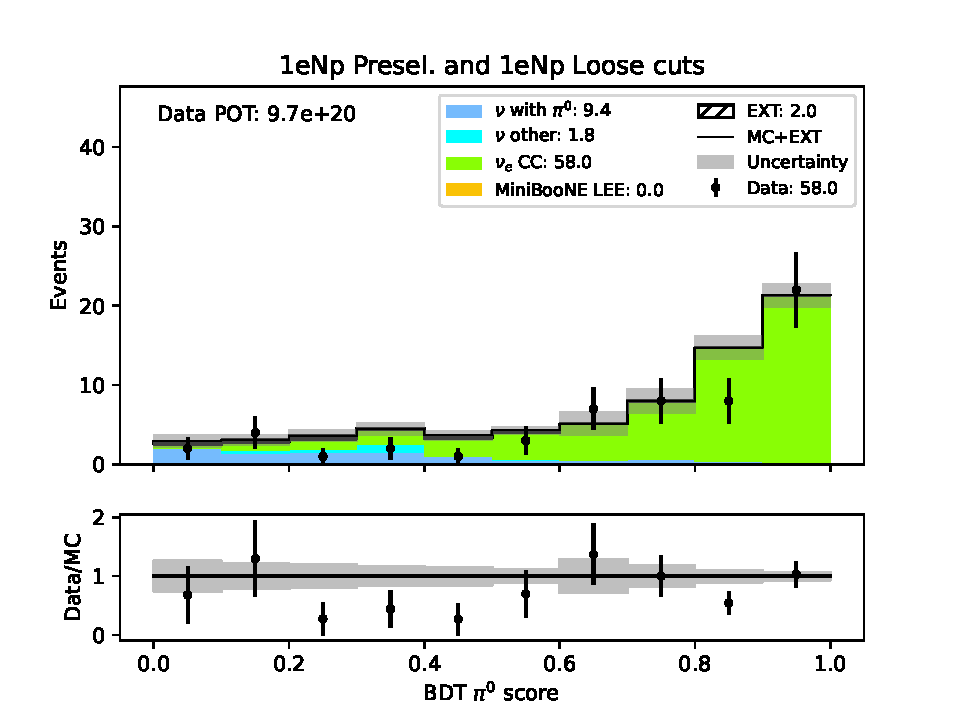
\includegraphics[width=\linewidth]{technote/Sidebands/Figures/ShowerEnergySideband/shr_energy_sideband_pi0_score_run1234b4c4d_NP_NPL.pdf}%
        \caption{$\pi^0$ score.}
    \end{subfigure}%
    \begin{subfigure}{0.5\linewidth}
        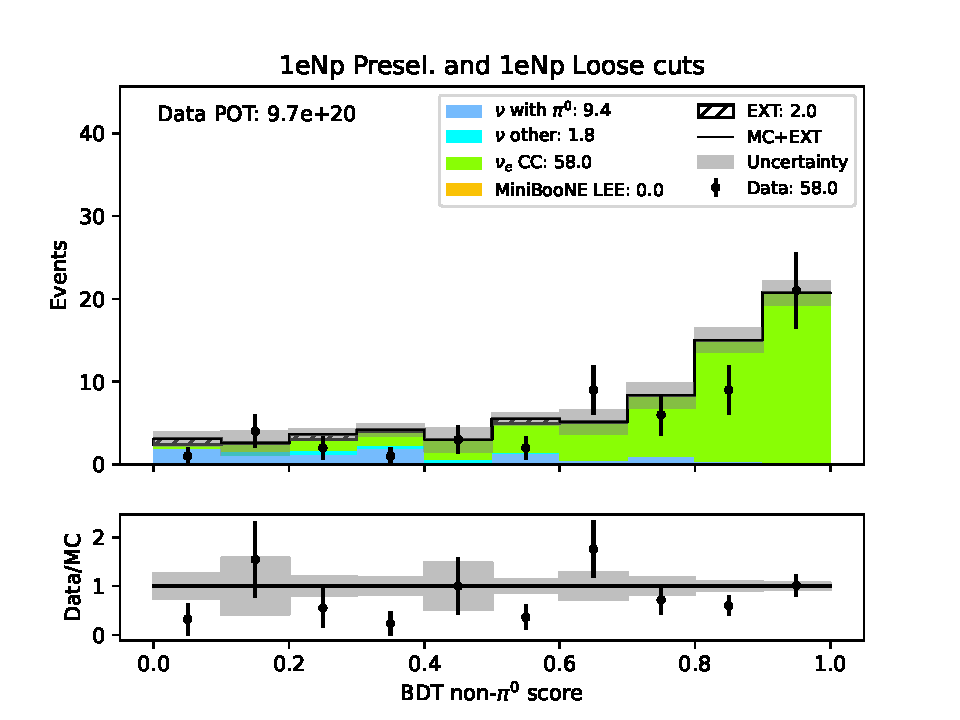
\includegraphics[width=\linewidth]{technote/Sidebands/Figures/ShowerEnergySideband/shr_energy_sideband_nonpi0_score_run1234b4c4d_NP_NPL.pdf}%
        \caption{Non-$\pi^0$ score.}
    \end{subfigure}
    \begin{subfigure}{0.5\linewidth}
        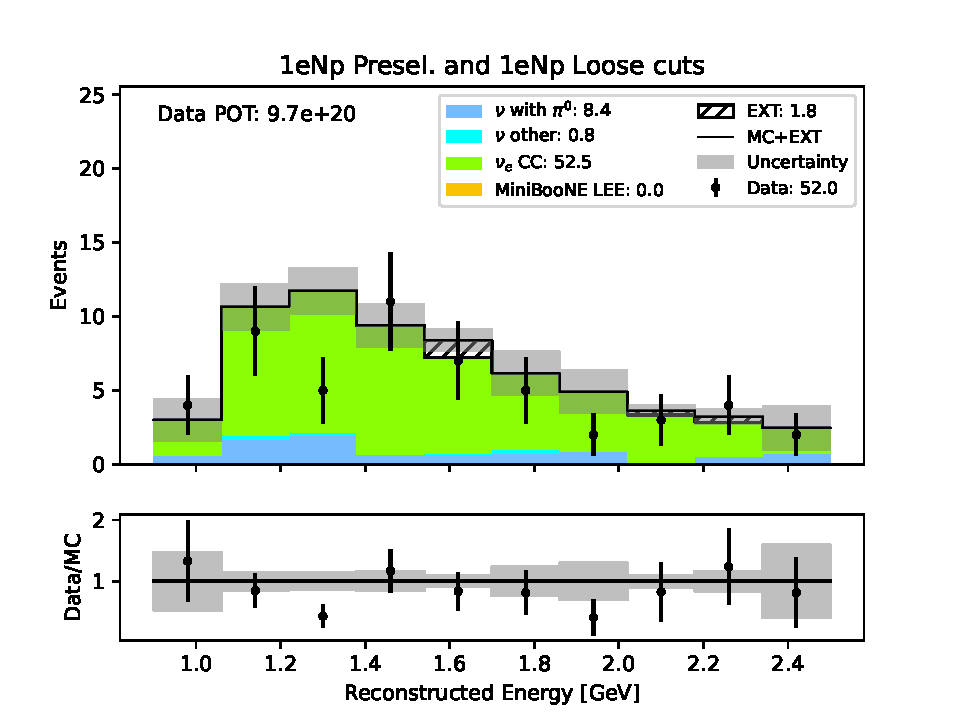
\includegraphics[width=\linewidth]{technote/Sidebands/Figures/ShowerEnergySideband/shr_energy_sideband_reco_e_run1234b4c4d_NP_NPL.pdf}%
        \caption{Reconstructed neutrino energy.}
    \end{subfigure}
    \caption{Results of applying the loose 1eNp event selection to the high shower energy sideband. Data from runs 1-5 shown.}
    \label{fig:ShrEnergySideband1eNpRuns12345}
\end{figure}

\begin{figure}[H]
    \centering
    \begin{subfigure}{0.5\linewidth}
        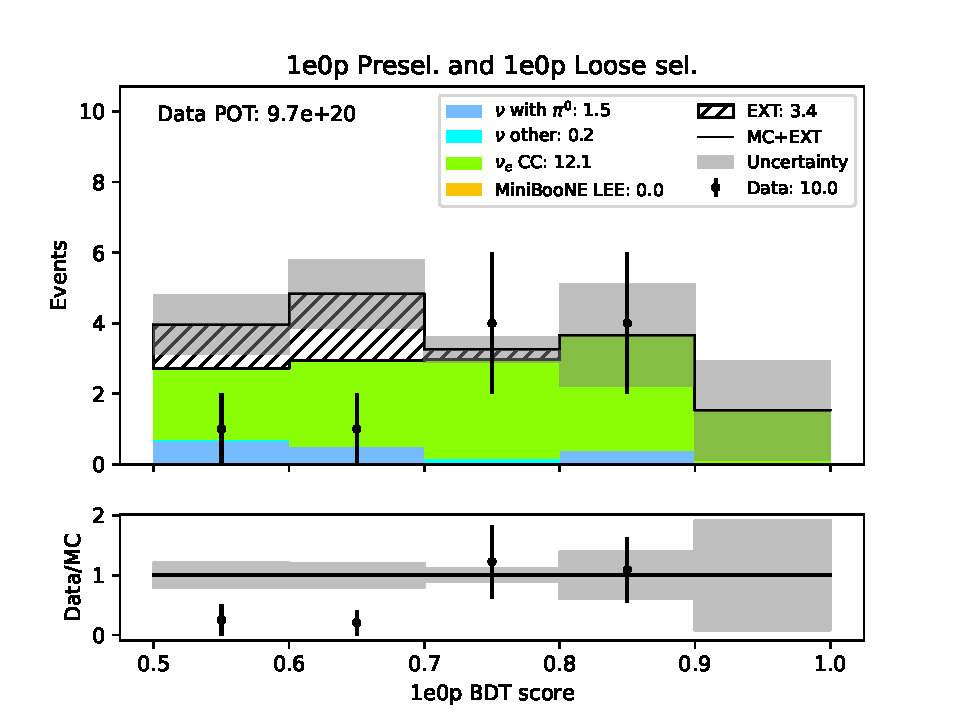
\includegraphics[width=\linewidth]{technote/Sidebands/Figures/ShowerEnergySideband/shr_energy_sideband_bkg_score_run1234b4c4d_ZP_ZPLOOSESEL.pdf}%
        \caption{Background score.}
    \end{subfigure}%
    \begin{subfigure}{0.5\linewidth}
        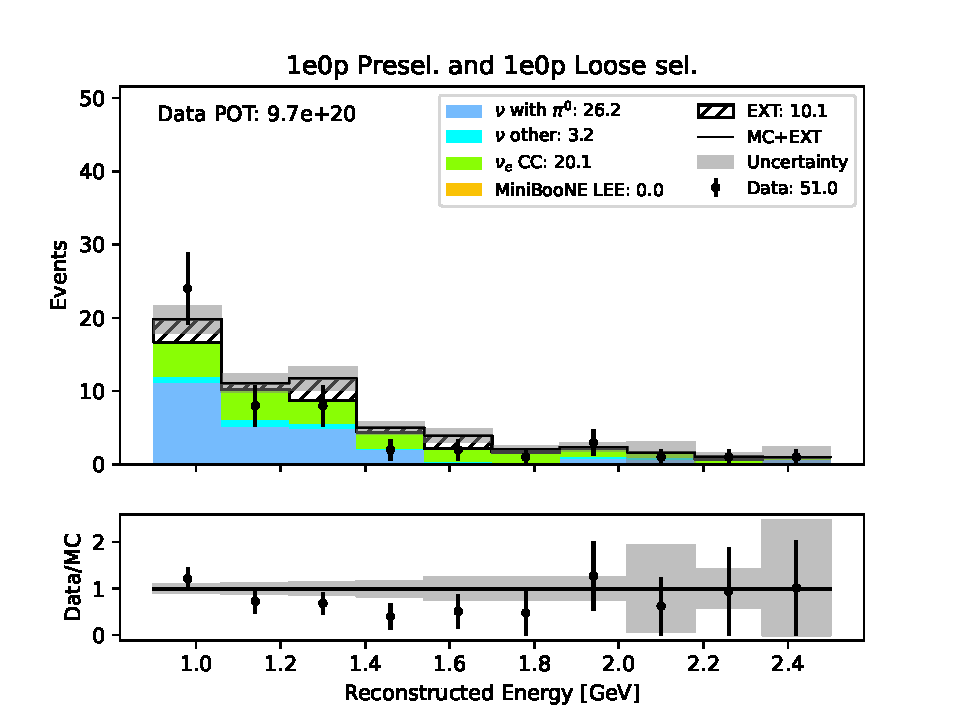
\includegraphics[width=\linewidth]{technote/Sidebands/Figures/ShowerEnergySideband/shr_energy_sideband_reco_e_run1234b4c4d_ZP_ZPLOOSESEL.pdf}%
        \caption{Reconstructed neutrino energy.}
    \end{subfigure}
    \caption{Results of applying the loose 1e0p event selection to the high shower energy sideband. Data from runs 1-5 shown.}
    \label{fig:ShrEnergySideband1e0pRuns12345}
\end{figure}

